\documentclass[11pt]{article}
\usepackage[margin=1in, headheight=14pt]{geometry}
\usepackage{amsmath, amssymb}
\usepackage{hyperref}
\usepackage{enumitem}
\usepackage{algorithm}
\usepackage{algpseudocode}
\usepackage{fancyhdr}
\usepackage{tcolorbox}
\usepackage{microtype}
\usepackage{tikz}
\usepackage{pgfplots}
\pgfplotsset{compat=1.18}
\usetikzlibrary{arrows.meta, positioning, calc, shapes.geometric}

\input{notation.tex}
\input{zk-notation.tex}
\input{environments.tex}
\input{lecture-macros.tex}

\pagestyle{fancy}
\fancyhf{}
\lhead{EECS 498/CSE 598: Zero-Knowledge Proofs}
\rhead{Winter 2026}
\lfoot{Lecture 21: Zero-Knowledge Middleboxes and TLS Oracles}
\rfoot{\thepage}
\renewcommand{\headrulewidth}{0.4pt}
\renewcommand{\footrulewidth}{0.4pt}

% Lecture-specific macros
\tcbuselibrary{skins, breakable}

\newtcolorbox{highlight}[1][]{
  colback=blue!5!white,
  colframe=blue!60!black,
  fonttitle=\bfseries,
  #1
}

\newtcolorbox{graybox}[1][]{
  colback=gray!8,
  colframe=gray!50,
  fonttitle=\bfseries,
  #1
}

\newcommand{\TLS}{\ensuremath{\mathsf{TLS}}}
\newcommand{\MPC}{\ensuremath{\mathsf{MPC}}}
\newcommand{\ZKMB}{\ensuremath{\mathsf{ZKMB}}}
\newcommand{\DoH}{\ensuremath{\mathsf{DoH}}}
\newcommand{\DoT}{\ensuremath{\mathsf{DoT}}}
\newcommand{\ZKTLS}{\ensuremath{\mathsf{zkTLS}}}

\begin{document}

%-----------------------------------------------------------------------
% Title Block
%-----------------------------------------------------------------------
\begin{center}
  {\LARGE \textbf{EECS 498 / CSE 598: Zero-Knowledge Proofs}}\\[6pt]
  {\large Winter 2026}\\[4pt]
  {\large \textbf{Lecture 21: Zero-Knowledge Middleboxes and TLS Oracles}}\\[4pt]
  {\large Instructor: Paul Grubbs \quad
    \href{mailto:paulgrub@umich.edu}{\texttt{paulgrub@umich.edu}} \quad
    Beyster 4709}
\end{center}

\vspace{0.5em}
\hrule
\vspace{1em}

%-----------------------------------------------------------------------
% Agenda
%-----------------------------------------------------------------------
\section*{Agenda}
\begin{itemize}
  \item Privacy and policy enforcement
  \item Zero-knowledge middleboxes for encrypted DNS
  \item TLS oracles and \ZKTLS
\end{itemize}

\hrule
\vspace{1em}

%-----------------------------------------------------------------------
\section{Privacy and Policy Enforcement}
%-----------------------------------------------------------------------

Modern network encryption hides application data and increasingly also hides
application metadata.  A client and server establish a shared key, for example
through a \TLS~1.3 handshake, and then use that key to protect subsequent
traffic.  Recent deployments extend this protection beyond payloads and toward
metadata such as the application-layer destination.

Examples of metadata-hiding mechanisms include:
\begin{itemize}
  \item encrypted DNS through \DoH{} and \DoT,
  \item Oblivious \DoH,
  \item encrypted certificates in \TLS~1.3,
  \item Encrypted Client Hello (\algo{ECH}).
\end{itemize}

At the same time, many networks enforce usage policies by scanning traffic at
an in-network enforcement point.  Common policy tasks include DNS filtering,
data-loss prevention, intrusion detection, and malware scanning.  Encryption
and policy enforcement therefore pull in opposite directions: one hides the
traffic, while the other relies on visibility into that traffic.

\begin{highlight}[title={Design Requirements}]
A practical construction should satisfy four constraints:
\begin{enumerate}
  \item Standard encryption should remain unchanged.
  \item The network should still be able to enforce policies.
  \item The remote server should not need to change.
  \item Circumvention through independent ``inner'' encryption, such as VPNs
        or Tor, should remain possible.
\end{enumerate}
\end{highlight}

The fourth requirement separates policy enforcement from universal censorship.
The objective is local-policy compliance by default rather than elimination of
all client-initiated tunneling.

\begin{remark}
Prior proposals include multi-context \TLS, BlindBox, and SGX-based designs.
Zero-knowledge middleboxes preserve ordinary end-to-end encryption and move
policy enforcement into a zero-knowledge proof system.
\end{remark}

%-----------------------------------------------------------------------
\section{Zero-Knowledge Middleboxes}
%-----------------------------------------------------------------------

\begin{definition}[Zero-knowledge middlebox]
A zero-knowledge middlebox protocol is a policy-enforcement mechanism in which
the client enforces the policy locally and sends a zero-knowledge proof that
the encrypted traffic is compliant, while the middlebox verifies the proof and
blocks traffic if verification fails.
\end{definition}

The protocol is organized in four steps:
\begin{enumerate}
  \item On network join, the client receives a description of the policy.
  \item The client and server establish keys and encrypt traffic normally.
  \item The client checks the policy locally and proves a statement of the form
        ``the ciphertext contains compliant traffic.''
  \item The middlebox verifies the proof and blocks traffic on failure.
\end{enumerate}

\begin{center}
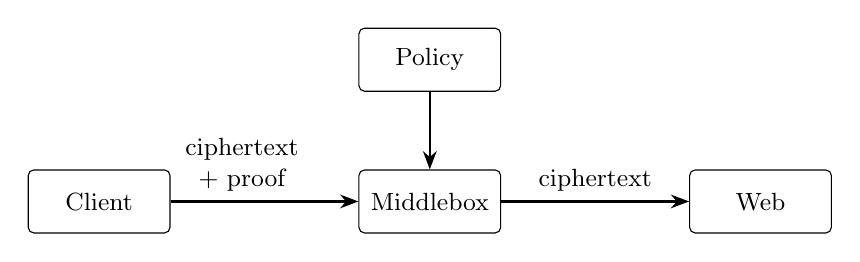
\begin{tikzpicture}[
  every node/.style={font=\small},
  box/.style={draw, rounded corners=2pt, minimum width=18mm, minimum height=8mm, align=center},
  arr/.style={-Stealth, thick}
]
  \node[box] (C) at (0,0) {Client};
  \node[box] (M) at (4.2,0) {Middlebox};
  \node[box] (S) at (8.4,0) {Web};
  \node[box] (P) at (4.2,1.8) {Policy};
  \draw[arr] (P) -- (M);
  \draw[arr] (C) -- node[above,align=center,pos=0.38] {ciphertext\\+ proof} (M);
  \draw[arr] (M) -- node[above] {ciphertext} (S);
\end{tikzpicture}

\smallskip
\emph{The middlebox checks compliance proofs without modifying the client-to-server
encryption protocol.}
\end{center}

\begin{proposition}
If the proof system is zero knowledge and sound, then the construction above
preserves the main design goals: encryption is unchanged, policy enforcement is
retained, and the remote server does not need to process proofs.
\end{proposition}

\begin{proof}[Proof sketch]
The server sees only the ordinary encrypted traffic because the proof is
checked locally by the middlebox.  Soundness guarantees that accepted traffic
satisfies the policy.  Zero knowledge guarantees that the proof reveals no
information beyond policy compliance.
\end{proof}

\begin{remark}
Policies with very large circuit complexity remain impractical.  A policy that
requires evaluating a large machine-learning model on every packet would force
that entire computation into the proof system.
\end{remark}

The key-schedule complexity is the central technical obstacle.  Efficient
middlebox proofs cannot treat \TLS~1.3 channel opening as a single symmetric
decryption call.  The witness key must be constrained to the actual
handshake-derived traffic secret obtained from the \TLS~1.3 key schedule, which
expands $\mathsf{PSK}$ and $\mathsf{DHE}$ through intermediate secrets such as
$\mathsf{ES}$, $\mathsf{HS}$, and $\mathsf{MS}$ before producing the client and
server traffic secrets.

\begin{center}
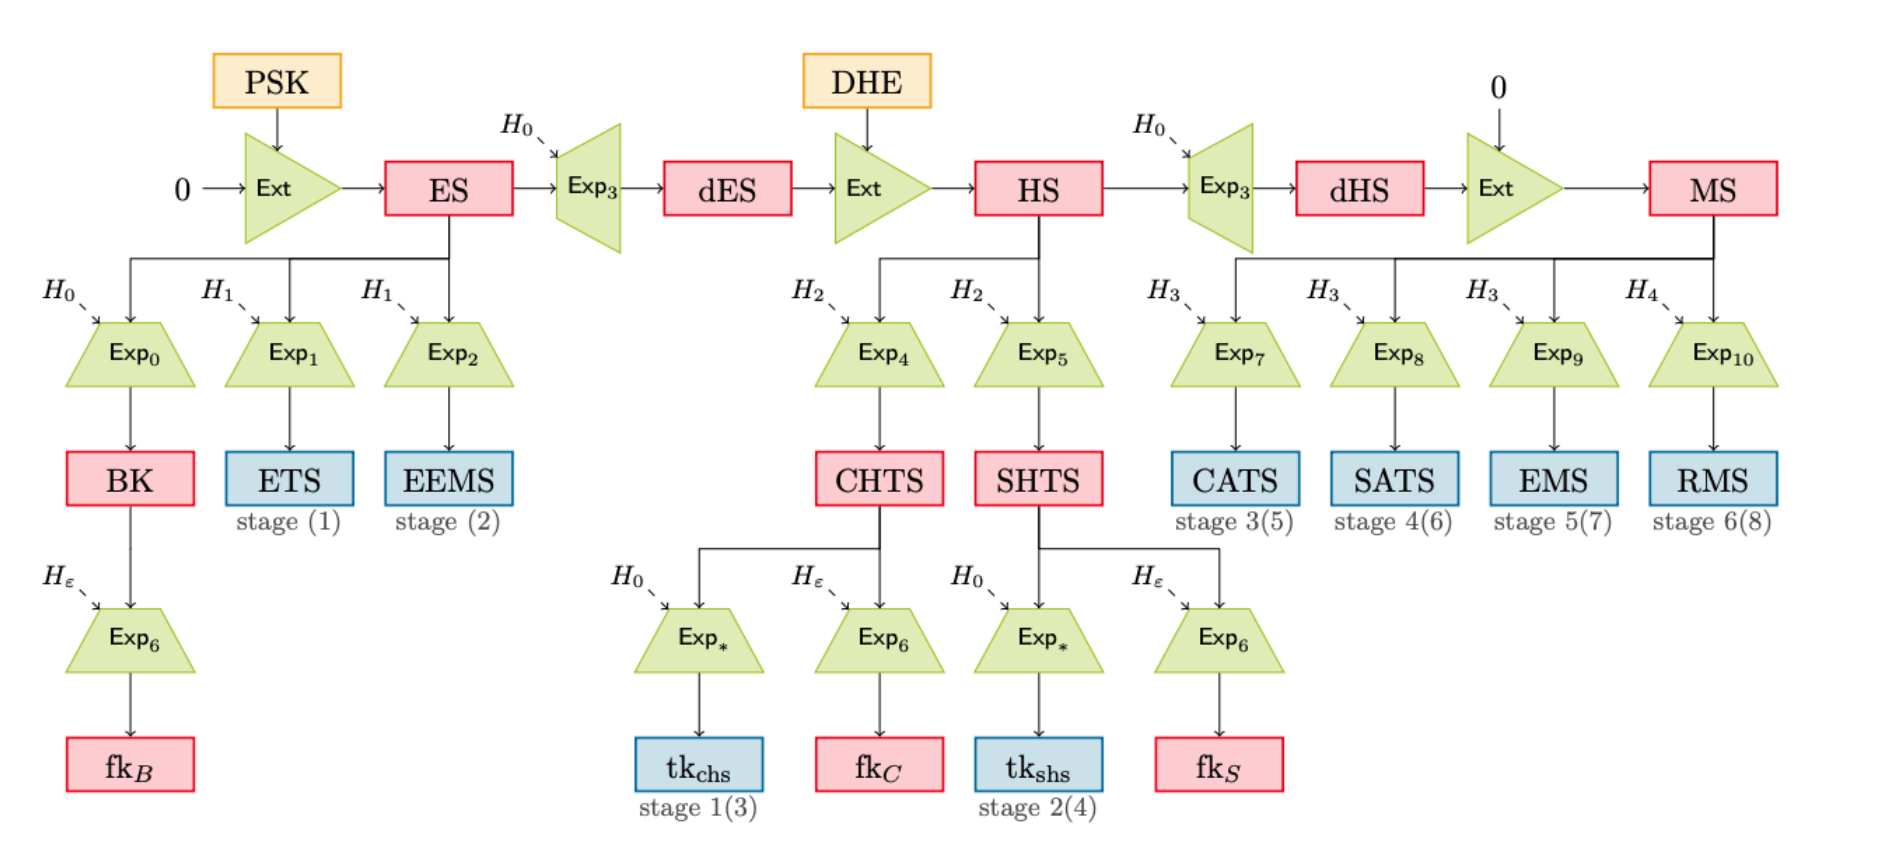
\includegraphics[width=0.94\textwidth]{figures/lecture21-tls13-key-schedule-final.png}

\smallskip
\emph{\TLS~1.3 key schedule for deriving the traffic secrets used in channel
opening.}
\end{center}

%-----------------------------------------------------------------------
\section{Circuits for Zero-Knowledge Middleboxes}
%-----------------------------------------------------------------------

The proof system is expressed as a circuit with public input $\mathrm{In}$ and
witness $W$.
The prover computes
\[
  \pi \leftarrow \algo{Prove}(\text{Circuit}, \mathrm{In}, W),
\]
and the middlebox checks
\[
  b \leftarrow \algo{Verify}(\text{Circuit}, \mathrm{In}, \pi)
  \in \{0,1\}.
\]

For a middlebox application, the circuit decomposes into three stages:
\begin{enumerate}
  \item Channel Opening: decrypt the ciphertext and recover the plaintext.
  \item Parse + Extract: deserialize the relevant field from the plaintext.
  \item Policy Check: verify that the extracted data is policy compliant.
\end{enumerate}

\begin{center}
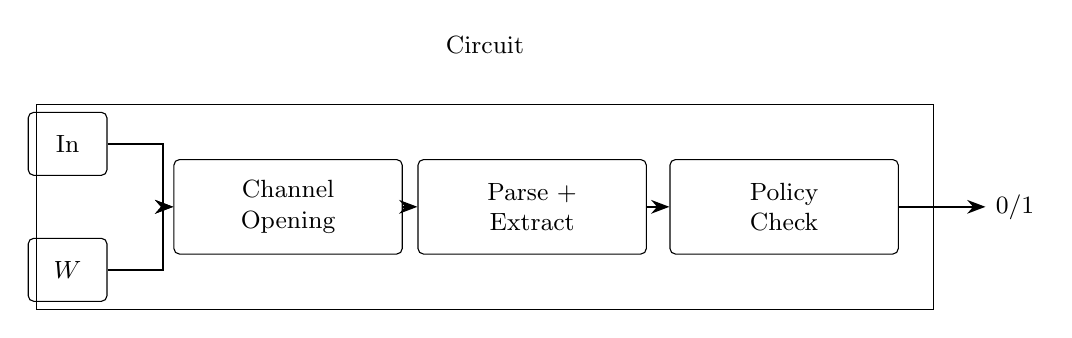
\begin{tikzpicture}[
  every node/.style={font=\small},
  box/.style={draw, rounded corners=2pt, minimum width=29mm, minimum height=12mm, align=center},
  io/.style={draw, rounded corners=2pt, minimum width=10mm, minimum height=8mm, align=center},
  arr/.style={-Stealth, thick}
]
  \node[draw, minimum width=114mm, minimum height=26mm] (Outer) at (3.7,0) {};
  \node at (3.7,2.05) {Circuit};
  \node[io] (In) at (-1.6,0.8) {$\mathrm{In}$};
  \node[io] (W) at (-1.6,-0.8) {$W$};
  \node[box] (O) at (1.2,0) {Channel\\Opening};
  \node[box] (P) at (4.3,0) {Parse +\\Extract};
  \node[box] (C) at (7.5,0) {Policy\\Check};
  \draw[arr] (In.east) -- ++(0.7,0) |- (O.west);
  \draw[arr] (W.east) -- ++(0.7,0) |- (O.west);
  \draw[arr] (O) -- (P);
  \draw[arr] (P) -- (C);
  \draw[arr] (C.east) -- ++(1.1,0) node[right] {$0/1$};
\end{tikzpicture}

\smallskip
\emph{A middlebox circuit opens the encrypted channel, extracts the relevant
field, and checks policy compliance.}
\end{center}

\subsection{Channel Opening for \texorpdfstring{\TLS~1.3}{TLS 1.3}}

The first task is to open a \TLS~1.3 ciphertext inside the circuit.  A natural
first attempt is to check
\[
  m \leftarrow \algo{TLS1.3Decrypt}(k, c),
\]
where $c$ is the ciphertext and $k$ is a witness key.

\begin{remark}
\TLS~1.3 \algo{AEAD} ciphertexts are not binding enough for this purpose.
A ciphertext can admit multiple valid decryptions under different keys.  A
client could therefore try to prove compliance for a plaintext opened under a
key unrelated to the connection observed on the wire.
\end{remark}

The repair is a key-consistency check.  The public input contains the
ciphertext together with handshake data, the witness contains the connection
key $k$, and the circuit accepts only if $k$ is an output of the observed
handshake.  The combination of the handshake transcript and the derived key is
then binding to the opened plaintext.

\begin{proposition}
If the circuit checks both decryption and consistency of the witness key with
the observed handshake, then a sound proof cannot certify a plaintext opened
under an unrelated key.
\end{proposition}

\begin{proof}[Proof sketch]
Any accepting proof must provide a witness key that satisfies the handshake
constraints.  Replacing the real connection key by an unrelated key would
violate those constraints unless the proof system's soundness were broken.
\end{proof}

\subsection{Key Consistency and Amortization}

The simplest key-consistency check reruns most of the client's key derivation
inside the circuit.  Diffie--Hellman values are binding to the shared secret,
so this approach is correct but expensive.  The more efficient construction
uses the observation that the handshake already commits to intermediate steps
of the key schedule.  Checking those intermediate commitments shortcuts most of
the derivation work.

The check can also be amortized across an entire session.  A \TLS~1.3 session
typically reuses the same traffic key across many records, so the expensive
consistency proof is needed only once.  Later proofs reuse a cached digest
\[
  h = \algo{Hash}(k).
\]

\begin{graybox}[title={Amortized Channel-Opening Rule}]
After the session setup has established a committed digest $h$:
\begin{enumerate}
  \item the public input contains $(c,h)$;
  \item the witness contains the session key $k$;
  \item the circuit checks
        \[
          m \leftarrow \algo{TLS1.3Decrypt}(k,c)
          \qquad\text{and}\qquad
          \algo{Hash}(k) = h.
        \]
\end{enumerate}
\end{graybox}

The middlebox stores $h$ once the session-level proof has verified, and later
record-opening proofs reuse that cached value.

%-----------------------------------------------------------------------
\section{Encrypted DNS and DNS Filtering}
%-----------------------------------------------------------------------

The Domain Name System maps names such as \texttt{example.com} to network-layer
addresses.  In traditional deployments, the local network resolver sees those
queries directly.  Encrypted DNS changes that arrangement by sending DNS
queries to a trusted resolver over \TLS~1.3, usually through \DoH{} or \DoT.

This design bypasses the local network's resolver and hides the contents of DNS
queries from the network.  Major browsers such as Firefox, Chrome, and Edge
enable encrypted DNS by default.  The privacy gain is immediate, but the local
network can no longer inspect DNS traffic and therefore cannot apply ordinary
DNS-filtering policies.

Some networks are legally required to filter Internet access.  A standard
example is the Children's Internet Protection Act, which requires certain
school and library networks to block or filter Internet access.  Browser
vendors therefore included downgrade mechanisms that allow a local network to
disable encrypted DNS.

The zero-knowledge-middlebox construction for encrypted DNS proceeds as
follows:
\begin{enumerate}
  \item The network creates a DNS blocklist together with a circuit.
  \item On network join, the client receives the circuit and the blocklist.
  \item The client performs a \TLS~1.3 handshake with the remote resolver.
  \item For each DNS query, the client sends the query ciphertext together with
        a proof of policy compliance.
\end{enumerate}

\begin{center}
\begin{minipage}{0.78\textwidth}
\centering
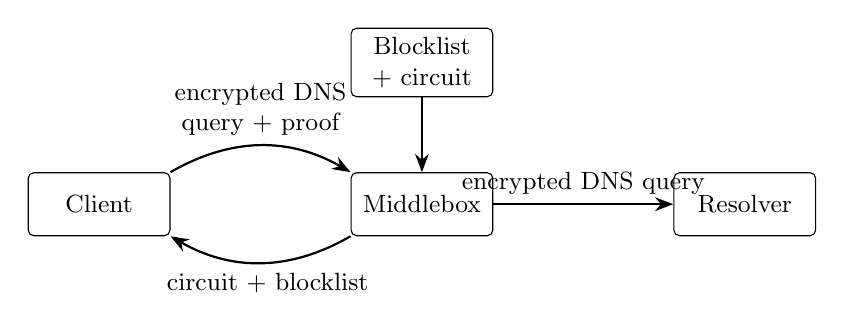
\begin{tikzpicture}[
  every node/.style={font=\small},
  box/.style={draw, rounded corners=2pt, minimum width=18mm, minimum height=8mm, align=center},
  arr/.style={-Stealth, thick}
]
  \node[box] (C) at (0,0) {Client};
  \node[box] (M) at (4.1,0) {Middlebox};
  \node[box] (S) at (8.2,0) {Resolver};
  \node[box] (B) at (4.1,1.8) {Blocklist\\+ circuit};
  \draw[arr] (B) -- (M);
  \draw[arr] (M.south west) to[out=210,in=330] node[below,pos=0.46] {circuit + blocklist} (C.south east);
  \draw[arr] (C.north east) to[out=30,in=150] node[above, align=center,pos=0.50] {encrypted DNS\\query + proof} (M.north west);
  \draw[arr] (M) -- node[above] {encrypted DNS query} (S);
\end{tikzpicture}

\smallskip
\emph{Encrypted DNS filtering with a zero-knowledge middlebox.}
\end{minipage}
\end{center}

The circuit structure matches the general \ZKMB{} pattern:
\begin{itemize}
  \item channel opening decrypts the DNS query;
  \item parse and extract deserializes the queried domain name;
  \item policy check proves that the queried domain is not in the blocklist.
\end{itemize}

The non-membership proof uses a sorted Merkle tree over the blocklist.  To show
that a queried domain $d$ is not blocked, the prover supplies Merkle paths for
the predecessor and successor of $d$ in the sorted order and proves
\[
  d_{\mathrm{pred}} < d < d_{\mathrm{succ}}.
\]
This yields a succinct set non-membership proof for a static blocklist.

\begin{remark}
\DoH{} and \DoT{} differ in packet format, so the parse-and-extract circuit is
slightly different across the two protocols.  Protecting the privacy of the
blocklist itself requires stronger tools, for example private-set-intersection
style techniques, than the basic static-Merkle construction.
\end{remark}

%-----------------------------------------------------------------------
\section{Experimental Results}
%-----------------------------------------------------------------------

The reported prototype measurements use Groth16 and eight threads.  The
key-consistency proof is a once-per-session setup cost; the DNS case studies
exclude that setup.

\begin{center}
\small
\renewcommand{\arraystretch}{1.1}
\setlength{\tabcolsep}{5pt}
\begin{tabular}{lrrrrr}
\multicolumn{6}{c}{Key Consistency Proof (once per session)}\\[0.3em]
\hline
Method & \#Gates (mil) & Prv time (s) & SRS (MB) & Proof size (b) & Vf time (ms) \\
\hline
Baseline  & 7.5 & 94.0 & 1200 & 128 & $\sim 5$ \\
Optimized & 1.1 & 16.5 & 149  & 128 & $\sim 5$ \\
\hline
\end{tabular}
\end{center}

\begin{center}
\small
\renewcommand{\arraystretch}{1.1}
\setlength{\tabcolsep}{4pt}
\begin{tabular}{lrrrrrr}
\multicolumn{7}{c}{DNS Case Studies (excluding once-per-session setup)}\\[0.3em]
\hline
Case Study & Ctxt size & \#Gates (k) & Prv time (s) & SRS (MB) & Proof size (b) & Vf time (ms) \\
\hline
\DoH{} (AES)    & 500 & 495 & 6.8 & 75 & 128 & $\sim 5$ \\
\DoT{} (ChaCha) & 255 & 195 & 3.1 & 32 & 128 & $\sim 5$ \\
\hline
\end{tabular}
\end{center}

The optimized key-consistency construction reduces the gate count by roughly
$7\times$, the prover time by roughly $6\times$, and the structured reference
string size by roughly $8\times$ relative to the baseline.  The \DoT{} case
study reaches a proof time of approximately $3.1$ seconds.

\begin{remark}
The dominant setup cost is the arithmetic representation of cryptographic
operations, especially hash evaluation inside \algo{R1CS}.  Multiple
middleboxes observing the same encrypted connection could in principle share
most of the channel-opening cost and repeat only the policy-specific portion.
\end{remark}

%-----------------------------------------------------------------------
\section{TLS Oracles and \texorpdfstring{\ZKTLS}{zkTLS}}
%-----------------------------------------------------------------------

Zero-knowledge middleboxes address policy enforcement for traffic originating
inside the network.  TLS oracles and \ZKTLS{} address a complementary problem:
allowing a client to prove something about data received from a web server.

A standard example is outsourced attestation.  A user may want to convince a
stock-trading platform that a bank account balance exceeds \$5{,}000, even
though only the bank can authoritatively determine that balance.

Without legacy constraints, the cleanest solution is for the bank to sign
application-level claims directly.  TLS oracles are needed because most
deployed services do not export such signatures.

The main design constraints in this setting are:
\begin{enumerate}
  \item no inline third party should be required;
  \item the relying party should still obtain authenticity of the exported
        claim;
  \item privacy may be desirable, but authenticity is the first objective and
        zero knowledge can be layered on top.
\end{enumerate}

The standard high-level approach uses secure multiparty computation.  The
client and the relying party jointly emulate a \TLS{} client with \MPC.  When
the server sends encrypted data, the client and the relying party jointly
decrypt it through that shared \TLS{} client state.  Any later claim exported
by the client is therefore tied to a genuine server response rather than to a
client forgery.

\begin{proposition}[Informal role of MPC in TLS oracles]
The \MPC{} layer prevents unilateral client forgery by ensuring that the client
does not have sole control over the effective \TLS{} client state used to open
the server's ciphertexts.
\end{proposition}

\begin{proof}[Proof sketch]
If the client alone controlled the decryption state, then it could invent
claims about server responses without a verifiable link to the real server
transcript.  Joint emulation of the \TLS{} client makes response opening a
shared computation, so the relying party can trust that exported claims are
derived from authenticated server data.
\end{proof}

\begin{remark}
The distinction between the two settings is structural.  A \ZKMB{} certifies
compliance of outgoing traffic, whereas TLS oracles certify authenticity of
incoming data.
\end{remark}

\bigskip
\hrule
\bigskip

\begin{thebibliography}{9}

\bibitem{GrubbsEtAl22}
  P.~Grubbs, A.~Arun, Y.~Zhang, J.~Bonneau, and M.~Walfish,
  ``Zero-knowledge middleboxes,''
  \emph{USENIX Security}, 2022.

\bibitem{DowlingEtAl21}
  B.~Dowling, M.~Fischlin, F.~G\"unther, and D.~Stebila,
  ``A cryptographic analysis of the TLS 1.3 handshake protocol,''
  \emph{Journal of Cryptology}, 2021.

\end{thebibliography}

\end{document}
